\section{Общие сведения и первичный анализ данных}

\subsection{Общие сведения}

\textbf{Вариант:} A-5.\\
\textbf{Группа:} A.\\
\textbf{Объём выборки:} \(n = 54\).\\
\textbf{Уровень значимости:} \(\alpha = 0.05\).\\
\textbf{Фактор (объясняющая переменная):} \(x\) — скорость чтения SSD, МБ/с.\\
\textbf{Результат (зависимая переменная):} \(y\) — скорость записи SSD, МБ/с.\\
\textbf{Дополнительная модель:} степенная \(y = ax^b\).\\
\textbf{Прогнозное значение:} \(x^* = 1207.9904\).

\subsubsection{Источник данных}

Данные взяты из реального набора \texttt{openintro::ssd\_speed} — скорости чтения и записи твердотельных накопителей (SSD). Страница-источник: \texttt{https://vincentarelbundock.github.io/Rdatasets/doc/openintro/ssd\_speed.html}. В выборку включены все наблюдения исходного набора без дополнительных фильтров.

\subsubsection{Инструменты}

Все вычисления выполнены на языке Python. При оценивании параметров линейной и степенной (после линеаризации) моделей использовались непосредственные формулы МНК; параметры квадратичной модели оценены функцией \texttt{numpy.polyfit}. Доверительные интервалы и p-value вычислены с использованием \texttt{scipy.stats.t}. Графики построены библиотекой \texttt{matplotlib}.

\subsection{Описательные статистики}

В таблице~\ref{tab:desc} приведены основные числовые характеристики переменных.

\begin{table}[H]
\centering
\caption{Описательные статистики переменных}
\label{tab:desc}
\begin{tabular}{lcc}
\toprule
Показатель & \(x\) (чтение, МБ/с) & \(y\) (запись, МБ/с) \\
\midrule
Среднее (\(\bar{x}\), \(\bar{y}\)) & 1128.963 & 1090.963 \\
Минимум & 376.000 & 359.000 \\
Максимум & 2381.000 & 3144.000 \\
\bottomrule
\end{tabular}
\end{table}

\subsection{Диаграмма рассеяния и гипотеза о характере связи}

На рисунке~\ref{fig:scatter} представлена диаграмма рассеяния исходных данных.

\begin{figure}[H]
\centering
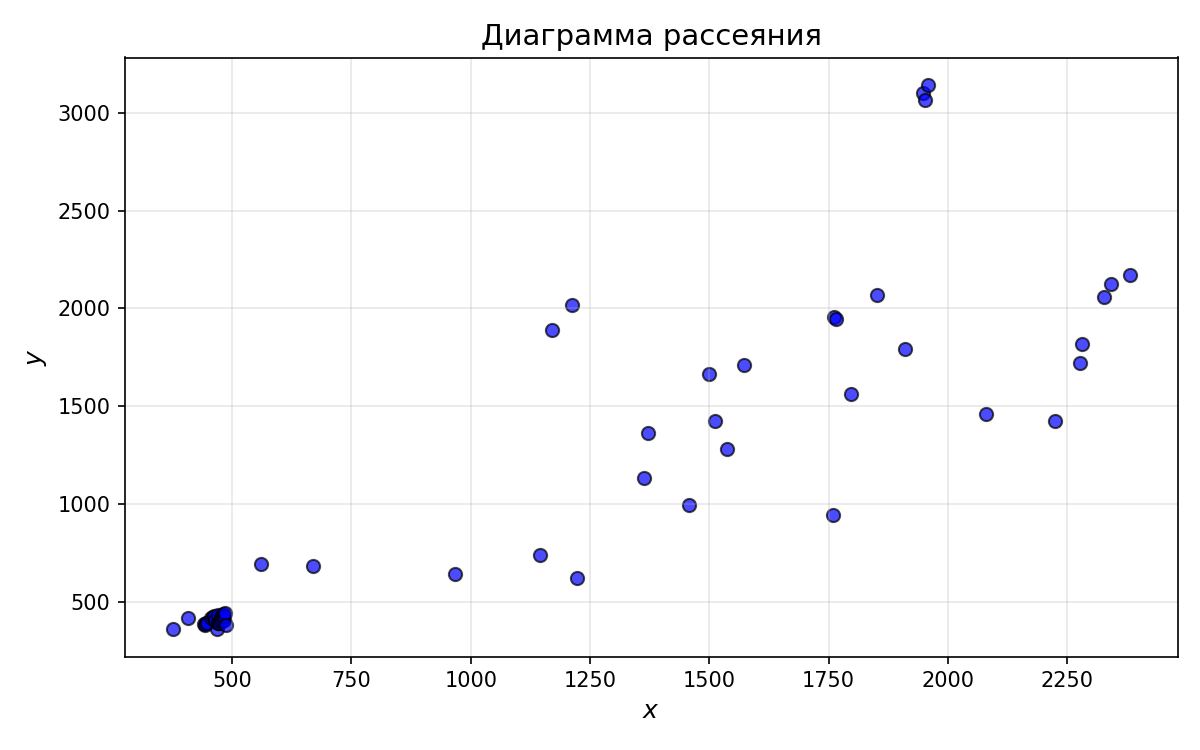
\includegraphics[width=0.75\textwidth]{scatter.png}
\caption{Диаграмма рассеяния \((x_i, y_i)\): скорость чтения и записи SSD}
\label{fig:scatter}
\end{figure}

По диаграмме рассеяния можно сделать следующие наблюдения:
\begin{itemize}
    \item наблюдается \textbf{положительная} связь между скоростью чтения \(x\) и скоростью записи \(y\): с ростом скорости чтения скорость записи в среднем увеличивается;
    \item характер связи близок к \textbf{линейному}, однако при больших значениях \(x\) разброс \(y\) заметно возрастает (гетероскедастичность);
    \item присутствует несколько точек с высокими значениями \(y\) при \(x > 1900\), которые могут оказывать существенное влияние на параметры модели.
\end{itemize}

\textbf{Предварительная гипотеза:} между скоростью чтения и скоростью записи SSD существует положительная зависимость, близкая к линейной; возможно также наличие слабой нелинейной составляющей. Для проверки гипотезы будут построены и сравнены три модели: линейная, квадратичная и степенная.

\subsection{Исходные данные}

В таблице~\ref{tab:data_sample} приведён фрагмент исходных данных (первые 10 наблюдений из 54).

\begin{table}[H]
\centering
\caption{Фрагмент исходных данных (первые 10 строк)}
\label{tab:data_sample}
\begin{tabular}{ccc}
\toprule
\(i\) & \(x_i\) (чтение, МБ/с) & \(y_i\) (запись, МБ/с) \\
\midrule
1 & 376.000 & 361.000 \\
2 & 408.000 & 419.000 \\
3 & 442.000 & 385.000 \\
4 & 443.000 & 381.000 \\
5 & 445.000 & 389.000 \\
6 & 448.000 & 390.000 \\
7 & 456.000 & 418.000 \\
8 & 459.000 & 420.000 \\
9 & 463.000 & 428.000 \\
10 & 465.000 & 407.000 \\
\bottomrule
\end{tabular}
\end{table}
